\chapter{Introduction}
\label{introduction}

\renewcommand{\thepage}{\arabic{page}} 			% arabic enumeration
\setcounter{page}{1}                   			% set page number 1

In these last years, a growing interest has been shown in robotics, In fact, several industries (automotive, medical, manufacturing, space, etc.), require robots to replace men in dangerous, repetitive or onerous situations. A wide area of this research is dedicated to Unmaned Aerial Vehicle (UAV) and especially the one of having the capability of Vertical TakeOff and Landing (VTOL) \cite{largeQuadrotor}. This kind of vehicle can be use in a variety of different scenario, for its reasonable price, small dimensions and great sensors capability. In particular, nowdays intensive research as been accomplish in the area of enviroment monitoring and exploration, accomplish with different strategies and sensors.

\begin{SCfigure}[\sidecaptionrelwidth][h]
	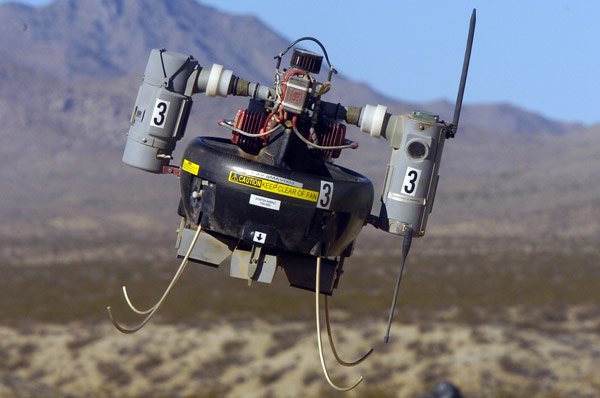
\includegraphics[scale=0.4]{images/fukushima.jpg}
	\caption{An example of UAV. T-Hawk, a US-made UAV, commonly used to search for roadside bombs in Iraq, made its debut when it photographed the Fukushima nuclear plant from above, providing a detailed look at the interior damage.}
	\label{fig:application}
\end{SCfigure}  

\noindent Many typse of UAVs have been developed over the last years, in particular the quadrotor type \cite{Aalborg}. The aim of this thesis is to contribute to the develop of the so called \textit{Prometheus project}, a fully autonomus vertical takeoff and landing vehicle, able to perform indoor enviroment exploration and mapping. To do this, we were inspired from the film Prometheus, where drones are able to map an indoor cave. Of course, due to technology and budget limitations, the vehicle will not have the same performance, but will have in theory the same capabilities. As previously said, this thesis is only a part of the project, that has been divided in three main parts:

\begin{itemize}
	\item mechanical design and building of the UAV \cite{Carlos};
	\item mathematical model, system identification and control;
	\item usage of the sensors, mapping and navigation algorithms.
\end{itemize}

\noindent This thesis will focus on the second point, but briefly introductions will give also in the other two points, in particular in the mechanical design, necessary for develop a mathematical model. 

\begin{SCfigure}[\sidecaptionrelwidth][h]
	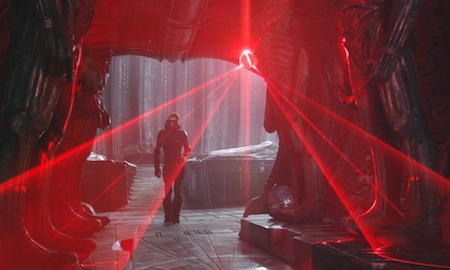
\includegraphics[scale=0.6]{images/prometheus_film.jpg}
	\caption{Frame of the prometheus movie, where the drone is performing the exploration and mapping of the cave.}
	\label{fig:prometheusFILM}
\end{SCfigure}

\noindent \textcolor{red}{Description of the varius chapters...}